\documentclass[a4paper,12pt]{ctexart}
\usepackage[style=gb7714-2015ay]{biblatex}
\usepackage{minted}
\usepackage{tikz}
\usepackage{pgfplots}
\pgfplotsset{compat=1.16}
\addbibresource{reference.bib}
\usepackage{graphicx}
\usepackage{float}
\usepackage{amsmath}
\usepackage{amssymb}
\usepackage{caption}
\usepackage{booktabs}
\usepackage{subcaption}
\usepackage[hidelinks]{hyperref}
\title{基于KMV模型上市中小企业信贷风险研究}
\author{董晨阳}
\date{\today}
\begin{document}
\maketitle
\section*{引言}
财务报表反映公司静态基本面,市场价格反映市场对公司未来的预期,所以基于基本面与市场面的双轮驱动框架更能准确度量信用风险,KMV模型便是其中之一。\citet{彭伟2012基于}利用KMV模型研究我国2008-2011年的上市中小企业的信贷风险,对KMV模型参数进行了改进,用违约距离刻画中小企业信贷违约风险大小,发现违约距离具有一定的风险预测能力。在此研究基础上,\citet{彭伟2012我国上市中小企业信贷风险研究}将违约距离作为因子引入到更广泛的回归模型中,发现包含违约距离的回归模型对中小上市企业违约的判断准确性高于不含违约距离的模型。其对中小上市企业信货风险的度量具有更好的判别效果,能够提高预警判别模型的判定效率。

\subsection*{KMV模型理论}

KMV模型由KMV公司提出,理论如图\ref{fig:bsm}所示。KMV模型提出于1993年,三个字母是三个创业者名字的首字母,成立以来一直默默无闻,后一举成名于安然倒闭事件。KMV在安然倒闭前约一年,就大幅调高安然公司的违约概率,完败三大评级公司,后在2002年被穆迪收购。
\begin{figure}[ht]
    \centering
    \includegraphics*[width=0.8\linewidth]{img/KMV.png}
    \caption{企业债券的价值}\label{fig:bsm}
\end{figure}

模型基于\citet{black1973pricing}和\citet{merton1974pricing}提出的BSM公式,因而包含了关于期权定价的所有基本假设,包括无交易成本与税收、相对静态的无风险收益率、无套利机会等等;此外公司资产价值小于违约点则会选择违约、企业的资产价值服从布朗运动。

模型的基本思路是:当企业期望市场价值$V$低于企业所需清偿的负债值$DP$时企业将发生违约。对公司价值和违约点的“距离”除以$V$,以对公司规模作了一个标准化,便于建立不同规模公司之间的对比;同时观察需要多少个$V$标准差的变化使得公司价值落在违约点以下,这就是到违约的距离。
\begin{equation}
    DD=\frac{V_A-DP}{V_A\sigma_A}\label{eq:dd}
\end{equation}
逐项来看公式(\ref{eq:dd}):
\begin{enumerate}
    \item 资产价值$V_A$和波动率$\sigma_A$的计算:将企业所有者权益视作欧式看涨期权,即\begin{equation*}
              E=\begin{cases}
                  V_A-D & V_A>D    \\
                  0     & V_A\le D
              \end{cases}
          \end{equation*}
          可以得到\begin{eqnarray}
              E&=&VN(d_1)-e^{rT}DN(d_2)\label{eq:ee}\\
              \sigma_E&=&\frac{V_A}{V_E} \frac{\mathrm{d}E}{\mathrm{d}A}\sigma_A
          \end{eqnarray}其中$d_1=\frac{1}{\sigma_E\sqrt{T}}(\ln \frac{S}{L}+(\mu+\frac{1}{2}\sigma^2_E)T)$,$d_2=d_1-\sigma_E\sqrt{T}$
          所有者权益的价值和波动率都是公开的市场信息,从而可以计算得到$V_A$和$\sigma_A$
    \item $DP$的计算:违约点 D 需要考虑了流动性的影响,给长短债赋予不同的权重,将短期债务和长期债务考虑进去。KMV公司的计算方式为加总所有的短期负债(即到期日小于 1 年的)的面值加上 50\%长期债务的面值。
\end{enumerate}

得到违约距离$DD$后,KMV模型基于违约数据库,依据违约距离可以映射出公司实际的期望违约频率,例如历史上$DD=a$的公司有100个,其中有5个违约,那么$a$点的违约概率就为0.05。这种处理就对模型假设没有那么严格,也是与区别Merton模型最大的区别。 KMV 公司收集了包括3400上市公司和40000家非上市公司自1973年以来的资料,建立了庞大的数据库,得到从违约距离到预期违约率的映射关系,取得了良好的预测效果。

\citet{彭伟2012基于}对KMV模型的改进在于对违约点的估计不再只是长期负债一半加上短期负债,以公司ROA作为预期资产价值增长的速度$\mu$。

\subsection*{后验视角看KMV理论}

KMV模型运用了现代期权定价理论,建立违约预测模型,综合考虑了经验和模型,是对传统信用风险度量方法的一次重要革命。KMV 模型的信用风险衡量指标预期违约率主要来自股票市场价格变化的有关数据,可以及时反映信用风险水平的变化。该模型主要依赖股票市场数据和财务报表中的负债数据进行计算,能够防止会计信息失真对模型结果的影响。另外,股价中包含了投资者对于公司未来发展的预期,预期违约率中包含了投资者对信用状况未来发展趋势的判断,因此,该模型具有一定的前瞻性。国内对该模型的研究也比其他信用风险度量模型要多。

但KMV模型也存在一些缺陷。首先,模型的使用范围有一定的局限性。通常,该模型特别适用于上市公司的信用风险评估,而对非上市公司进行应用时,往往要借助一些会计信息或其他能够反映借款企业特征值的指标来替代模型中一些重要变量,同时还要通过对比分析最终得出该企业的期望违约概率,在一定程度上就有可能降低计算的准确性。其次,该模型假设公司的资产价值服从正态分布,而实际中企业的资产价值一般会呈现非正态的统计特征。再次,模型不能够对债务的不同类型进行区分,如偿还优先顺序、担保、契约等类型,使得模型的输出变量的计算结果不准确。

\section*{实证与复现}
\subsection*{数据预处理}

我国公开市场债券违约首现于2014年的11超日债违约,早于\citet{彭伟2012基于}写文章的日期。且截止至目前(\today),债券违约仍以非上市公司为主,如图\ref{fig:default}所示。因此\citet{彭伟2012基于}选择以公司是否被“ST”为违约标志。沪、深交易对财务状况和其他财务状况异常的上市公司的股票交易进行特别处理(Special Treatment),以表明比一般正常的上市公司具有较高的投资风险。实际情况中,虽然公司信贷违约与被 ST、*ST 不完全等同,但他们之间有较强的相关性,如超日债即为ST超日2011年发行的债券。
\begin{figure}[H]
    \centering
    \includegraphics*[width=\linewidth]{img/发行人首次债券违约.png}
    \caption{迄今为止发行人首次债券违约时间分布}\label{fig:default}
\end{figure}

采用是否ST衡量公司违约有一定的问题,这是由于当时数据的局限性造成的。但实施ST的原因与公司信贷违约尚有差距,如连续亏损、含非标意见等。尽管这些情形可能是公司走向违约等标志,但ST股票的判定和撤销取决于交易所的判断,交易所对风险的理解会影响到一家公司是否被ST。后验地看不少公司在公开市场违约时仍尚未被ST,如华夏幸福、泰禾、蓝光等企业,更遑论更一般的信贷市场违约(公开债务违约前往往是非公开债务如信托、银行贷款违约)时。时至今日我国信贷违约数据库尚在建设中,公开市场虽然打破了刚兑但数据量难以支撑大模型,这也是KMV模型应用的挑战之一。
\begin{table}[H]
    \centering
    \begin{tabular}{|c|c|c|}
        \hline
        符号   & 经营连续亏损 & 预警           \\\hline
        *ST  & 三年     & 退市预警         \\
        ST   & 二年     & 特别处理         \\
        S*ST & 三年     & 退市预警+还没有完成股改 \\
        SST  & 二年     & 特别处理+还没有完成股改 \\
        \hline
    \end{tabular}
    \caption{沪深交易所对ST/*ST的规定}
\end{table}

清理数据后,共有89家满足\citet{彭伟2012基于}中小企业的定义(原文中有111家):
\begin{enumerate}
    \item 2008 年 1 月 1 日之前在沪深证券交易所上市
    \item 流通股 ≤ 5 000 万股,且 2007 年 12 月31日前的主营收入或资产总额≤5 亿元。
    \item 删除那些停牌时间较长的公司,
    \item 没有 B 股、H 股股票
\end{enumerate}
数据描述性统计如图\ref{fig:des1}和图\ref{fig:des2}所示,其中波动率采用了GARCH(1,1)模型计算得出,公司权益的市场价值则针对我国国情。
\begin{figure}[H]
    \centering
    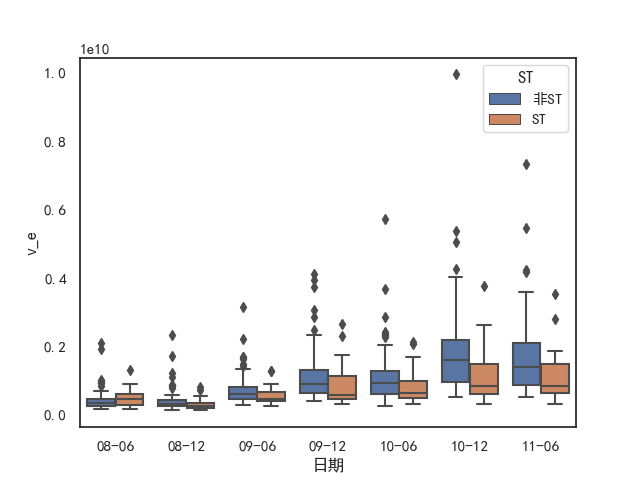
\includegraphics[width=0.8\textwidth]{img/v_e.png}
    \caption{股权价值}\label{fig:des1}
\end{figure}
\begin{figure}[H]
    \centering
    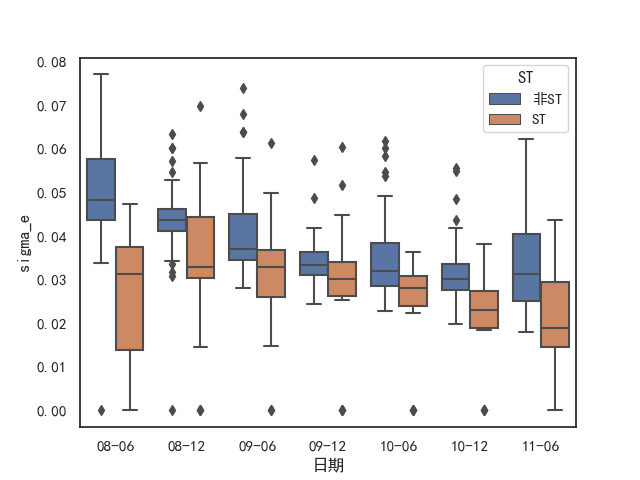
\includegraphics[width=0.8\textwidth]{img/sigma_e.png}
    \caption{股权价值波动率}\label{fig:des2}
\end{figure}

对于债权的价值,作者对所有08-11年的所有被实施ST的股票的总资产、短期负债和长期负债的价值进行了多元线性回归。复现结果如表\ref{tab:1}所示,与作者的$DPT = 1.11\times SD+0.65\times LD$接近,均大于KMV公司的原始数据,说明我国中小上市企业信贷风险相对国外更高。
\begin{table}[H]
    \centering
    \small\begin{center}
\begin{tabular}{lclc}
\toprule
\textbf{Dep. Variable:}    &       总资产        & \textbf{  R-squared (uncentered):}      &     0.968   \\
\textbf{Model:}            &       OLS        & \textbf{  Adj. R-squared (uncentered):} &     0.968   \\
\textbf{Method:}           &  Least Squares   & \textbf{  F-statistic:       }          &     4304.   \\
\textbf{Date:}             & Wed, 23 Nov 2022 & \textbf{  Prob (F-statistic):}          & 5.84e-211   \\
\textbf{Time:}             &     11:05:32     & \textbf{  Log-Likelihood:    }          &   -6294.1   \\
\textbf{No. Observations:} &         282      & \textbf{  AIC:               }          & 1.259e+04   \\
\textbf{Df Residuals:}     &         280      & \textbf{  BIC:               }          & 1.260e+04   \\
\textbf{Df Model:}         &           2      & \textbf{                     }          &             \\
\textbf{Covariance Type:}  &    nonrobust     & \textbf{                     }          &             \\
\bottomrule
\end{tabular}
\begin{tabular}{lcccccc}
               & \textbf{coef} & \textbf{std err} & \textbf{t} & \textbf{P$> |$t$|$} & \textbf{[0.025} & \textbf{0.975]}  \\
\midrule
\textbf{流动负债}  &       1.3733  &        0.033     &    41.761  &         0.000        &        1.309    &        1.438     \\
\textbf{非流动负债} &       0.8951  &        0.053     &    16.821  &         0.000        &        0.790    &        1.000     \\
\bottomrule
\end{tabular}
\begin{tabular}{lclc}
\textbf{Omnibus:}       & 174.038 & \textbf{  Durbin-Watson:     } &    1.984  \\
\textbf{Prob(Omnibus):} &   0.000 & \textbf{  Jarque-Bera (JB):  } & 3432.492  \\
\textbf{Skew:}          &   2.077 & \textbf{  Prob(JB):          } &     0.00  \\
\textbf{Kurtosis:}      &  19.579 & \textbf{  Cond. No.          } &     3.41  \\
\bottomrule
\end{tabular}
%\caption{OLS Regression Results}
\end{center}

Notes: \newline
 [1] R² is computed without centering (uncentered) since the model does not contain a constant. \newline
 [2] Standard Errors assume that the covariance matrix of the errors is correctly specified.
    \caption{债权价值复现}\label{tab:1}
\end{table}

最后,作者将负债的平均期限假定为一年,企业预期资产价值增长的速度为ROA。
\begin{figure}[H]
    \centering
    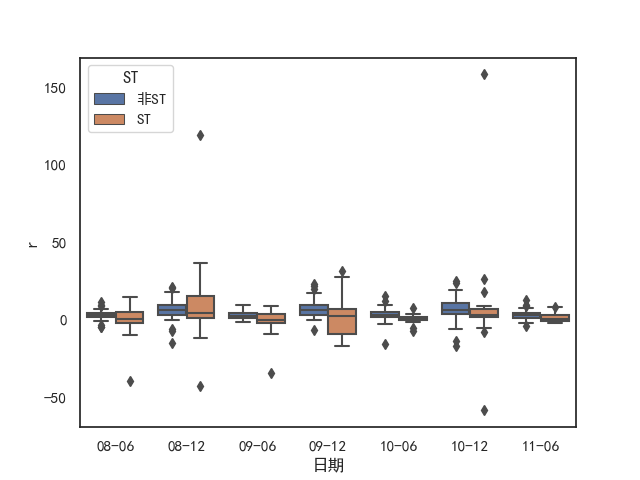
\includegraphics[width=0.8\textwidth]{img/r.png}
    \caption{ROA}
\end{figure}
\subsection*{中小上市企业的违约距离}
公式(\ref{eq:dd})和(\ref{eq:dd})可以进一步化简为
\begin{equation}
    DD=\frac{\ln \frac{V_A}{DPT}+(\mu-\frac{1}{2}\sigma^2)T}{\sigma_A\sqrt{T}}
\end{equation}

代入数据计算出违约距离如图\ref{fig:dd}所示,违约距离较低的如非ST股票在后来也逐渐沦为ST股票,如ST新智、ST冠福、ST天宏等。限于中国市场有限的违约率,我们难以通过违约距离$DD$直接得到相应的违约概率的历史映射,不过我们仍然可以从违约距离这一指标中窥见发行人的信用风险状况。
\begin{figure}[H]
    \includegraphics*[width=\linewidth]{img/dd.png}
    \caption{ST与非ST公司的违约距离}\label{fig:dd}
\end{figure}

而对KMV模型是否有效,作者采用了两个独立样本的K-S检验和Mann-Whitney检验,作者的K-S检验前 6 个半年及Mann-Whitney检验7个半年的P值均小于0.05,只有K-S 检验的 2011年上半年双尾检验概率 P 值为0.067。K-S检验的显著性差异证明ST与非ST公司的违约距离不是同一个分布,而但复现结果分别如表\ref{tab:KS}和表\ref{tab:MW}所示,显著性不强,仅在部分年份显著。
\begin{table}[H]
    \centering
    \begin{tabular}{lrrrrrrr}
\toprule
{} &  2008-06-30 &  2008-12-31 &  2009-06-30 &  2009-12-31 &  2010-06-30 &  2010-12-31 &  2011-06-30 \\
\midrule
statistic &    0.277778 &    0.222222 &    0.222222 &    0.194444 &    0.291667 &    0.291667 &    0.208333 \\
pvalue    &    0.236850 &    0.384915 &    0.384915 &    0.472853 &    0.206561 &    0.206561 &    0.427943 \\
\bottomrule
\end{tabular}

    \caption{两个独立样本的K-S检验}\label{tab:KS}
\end{table}
\begin{table}[H]
    \centering
    \begin{tabular}{lrrrr}
    \toprule
    {}        & 2008-06-30 & 2008-12-31 & 2009-06-30 & 2009-12-31 \\
    statistic & 158.000000 & 47.000000  & 135.000000 & 78.000000  \\
    pvalue    & 0.230442   & 0.005167   & 0.284836   & 0.028662   \\
    \midrule
    {}        & 2010-06-30 & 2010-12-31 & 2011-06-30 &            \\
    statistic & 182.000000 & 131.000000 & 217.000000 &            \\
    pvalue    & 0.443427   & 0.091772   & 0.892414   &            \\
    \bottomrule
\end{tabular}

    \caption{Mann-Whitney检验}\label{tab:MW}
\end{table}
% r有用吗
\section*{结论}
% 信贷市场违约模型的意义

经验与模型哪个重要正如剑宗与气宗之争,基本面重要还是市场面重要也正如哲学中唯物与唯心的探讨。不过我们认为,无论怎样,模型来源于经验的总结,最终也要回到经验中去,没有经验的模型如同空中楼阁,没有模型的经验也仅仅是有经历、无知识的简单再生产。所以我们一直以来都在结合经验与模型来对中国特色的信用市场进行分析,同时强调基本面与市场面结合交叉检验的风险分析框架,而本次提出的KMV模型正是结合了财务的基本面信息、权益市场信息(股价及其波动率)、债券市场信息(信用利差及基准利率),是为体现。
\nocite{*}
\appendix
\printbibliography%[heading=bibliography,title=参考文献]
\end{document}
